\documentclass{article}
\usepackage[utf8]{inputenc}
\usepackage{graphicx}
\usepackage{float}

\title{CR tp-simd}
\author{Chloé Dorchêne et Léo Marché}
\date{Janvier 2023}

\usepackage{geometry}
 \geometry{
 a4paper,
 left=30mm,
 right=30mm,
 top=30mm,
 }

\begin{document}

\maketitle

\section{Question 3}

\begin{figure}[h]
    \centering
    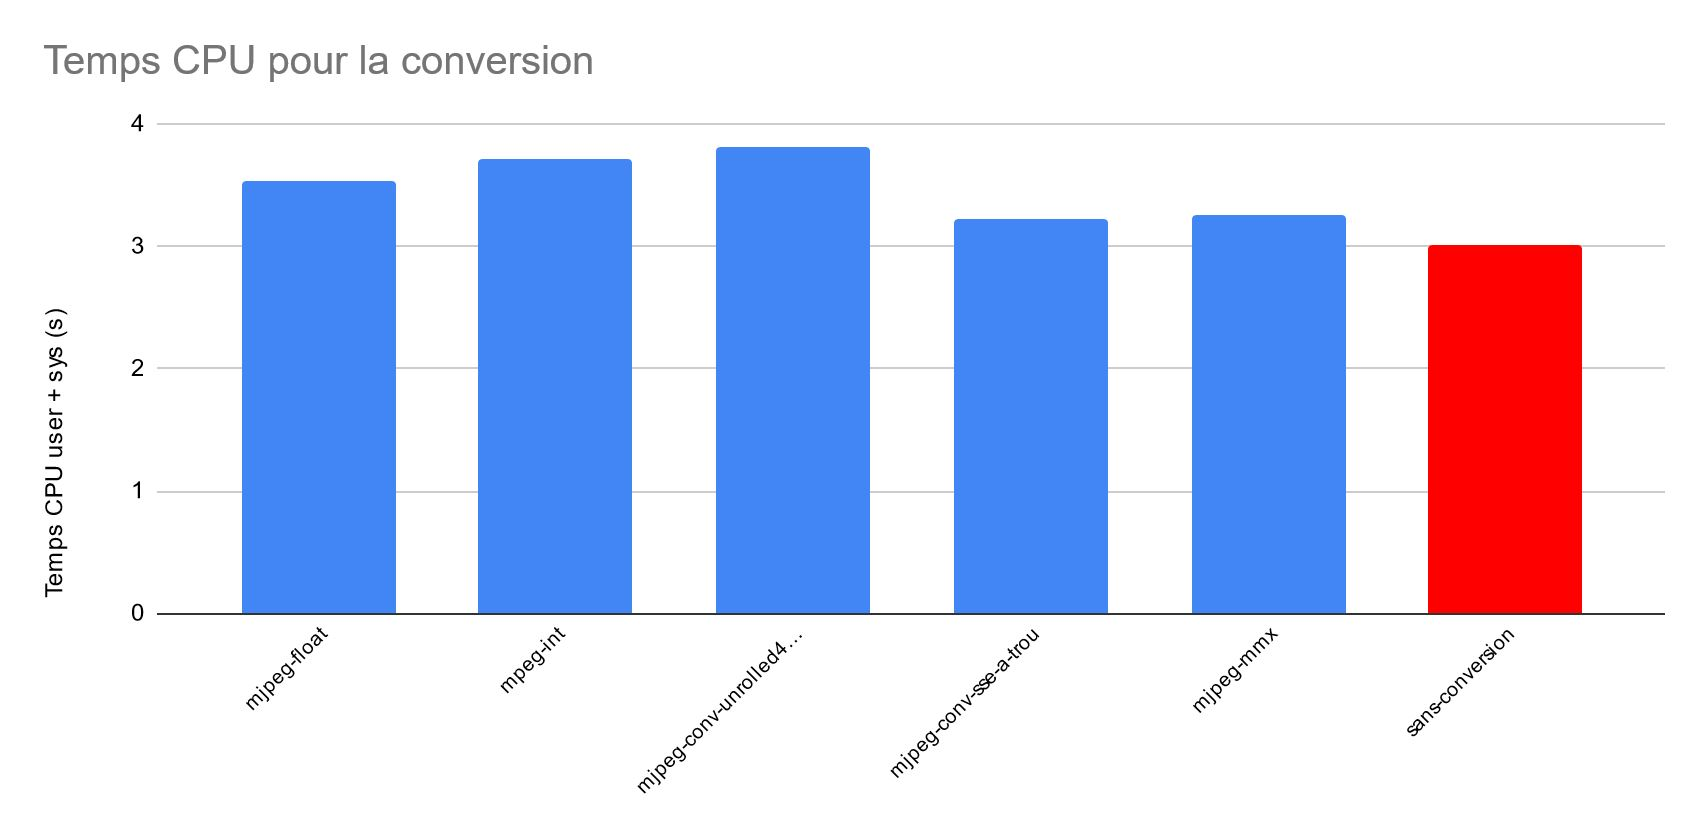
\includegraphics[width=0.9\linewidth]{temps_cpu_conversion.JPG}
    \caption{Temps CPU en fonction du convertisseur}
    \label{fig:comparaison}
\end{figure}

\begin{figure}[h]
    \centering
    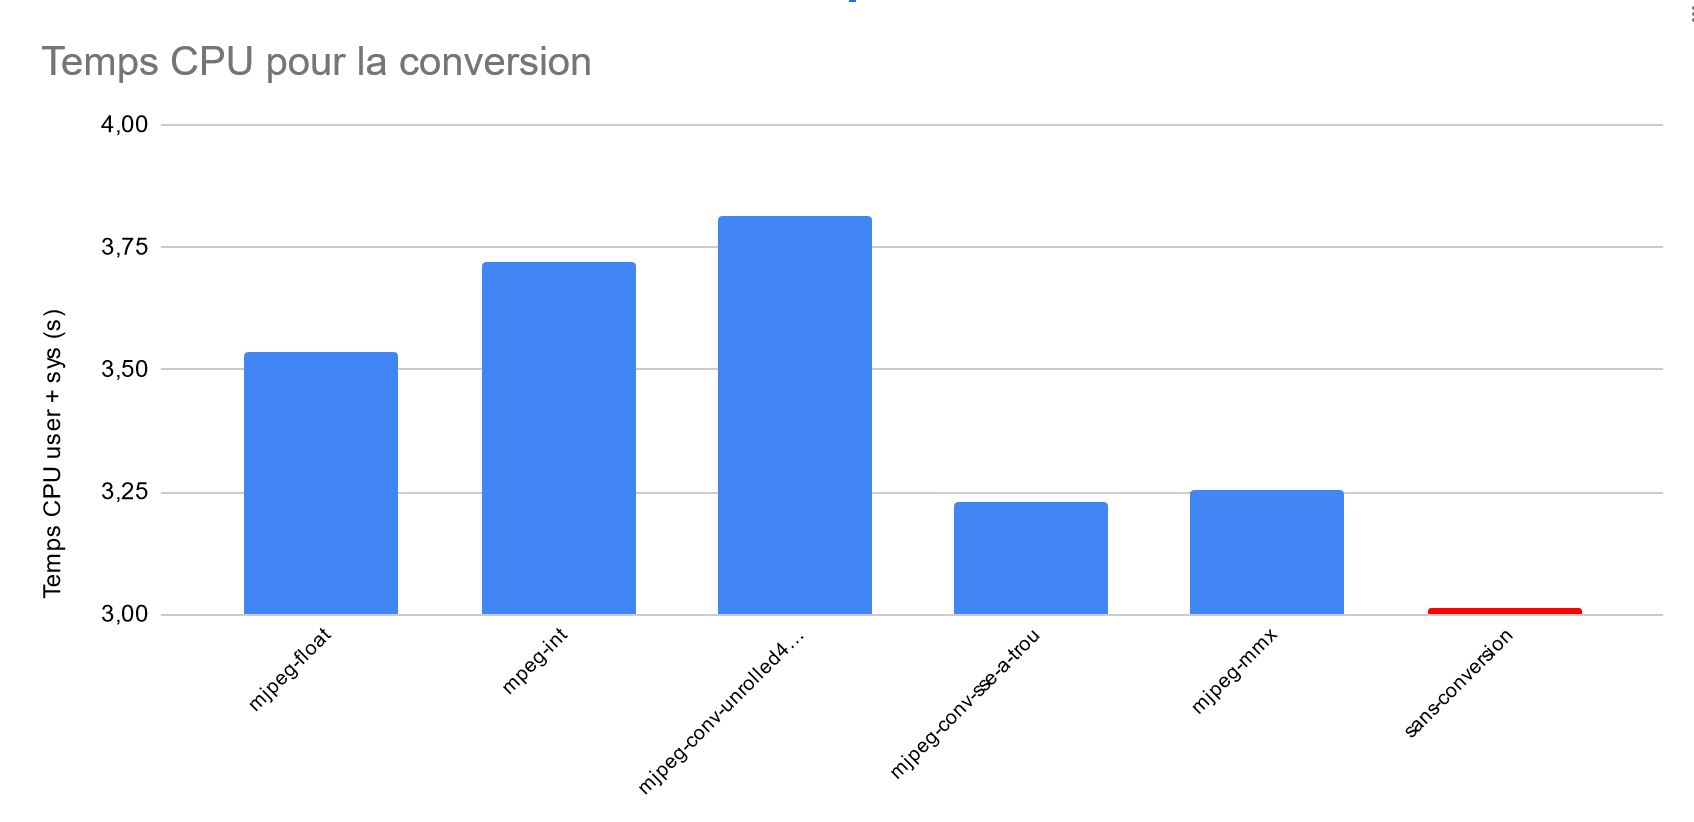
\includegraphics[width=0.9\linewidth]{temps_cpu_conversion_scaled.JPG}
    \caption{Temps CPU en fonction du convertisseur - Zoomé}
    \label{fig:comparaison2}
\end{figure}

Comme on peut le voir sur la figure \ref{fig:comparaison}, il semblerait qu'il y ait un offset incompressible en termes de temps CPU nécessaire à l'exécution. Cet offset vient probablement du temps de lecture du fichier vidéo et des autres conversions dans le pipeline de traitement vidéo.

Sur la figure \ref{fig:comparaison2} est représentée la comparaison des différents temps de calcul en prenant l'offset en compte. On remarque une très nette amélioration en utilisant les instructions SIMD (une division du temps de calcul par 2-3). Il est donc très intéressant des les utiliser pour les applications de traitement vidéo (lecteur, logiciel de montage, ...) d'exploiter les instructions SIMD.

Pour pousser l'expérience plus loin, on aurait pu essayer de comparer les performances de conversion avec une implémentation GPU.


\end{document}
